\section{Computational cost}
Training, scientific rollout, common scoring, saved-output analysis and paper
rendering are measured as separate activities. The two concurrent prediction
workers share fitted parameters but maintain separate map-query and history
state. Summed worker elapsed cost differs from concurrent wall throughput.
Execution-record and reconstruction details are collected in
Appendix~\ref{sec:execution-reconstruction}.


\section{Recorded environment and ordinary prediction-time examples}
\label{sec:preliminary-cost}\hypertarget{sec:preliminary-cost}{}
The recorded CPU environment has Windows 10, six physical and
12 logical CPUs, 31.73 GiB RAM, Python 3.10.13, NumPy 1.26.4 and PyTorch
2.3.1+cu121. The CUDA-enabled package name does not mean these CPU forecasts
used a GPU. Library threads are distinct from the two forecast workers;
the complete environment and thread settings are given in
Appendix~\ref{sec:runtime-record-details}.

\begin{table}[htbp]
\centering\small
\caption{Original ordinary prediction-time records at the first registered
primary origin and first RNG seed. One recorded run per row, not p50/p95
or an isolated latency comparison; no extra prediction was performed.
Seconds are rounded to three decimals for display only.}
\label{tab:preliminary-cost}\hypertarget{tab:preliminary-cost}{}
\begin{tabular}{@{}lr@{}}
\toprule
Configuration & Recorded prediction seconds\\
\midrule
Full01 & 0.973\\
GMM kernel & 0.817\\
dt300 & 0.862\\
EM & 0.676\\
MC & 0.572\\
\bottomrule
\end{tabular}
\end{table}
Each predicts the nominal 30-minute task with 512 paths and maximum 5-second
steps. The original \texttt{prediction\_seconds} field measures prediction
execution with inputs and models already prepared, not all recovery,
fitting, disk output, scoring or paper work. These five ordinary records
demonstrate that timing exists; a single run does not establish speedup,
tail latency or deployment cost. Full recorded precision is retained in
\path{paper/pirc17/preliminary-reader-presentation-v1.json}; it is not a claim
of microsecond measurement accuracy. The 75 cold and 75 warm trials and their
15 excluded warmups have all completed and appear in the original review
package; they are not replaced by this example table. Recorded elapsed
summaries do not certify uninterrupted isolated latency.


\section{Execution environment and timing boundary}
\label{sec:runtime-environment}\hypertarget{sec:runtime-environment}{}
Timed trials start with prepared causal inputs and fitted parameters already
resident. They include provider initialization, prediction setup, the full
rollout and prediction-time map reads and queries. Original input and
checkpoint preparation, fitting, offline scoring, artifact export and
validation, and provider teardown are outside this latency measurement;
their costs are not zero. Prediction latency, summed computation and
concurrent wall-clock completion time therefore answer different questions.

The isolated runtime experiment uses all ten terrain configurations and five
registered method subjects at the first primary origin and seed. Each condition
has five provider-cold trials, one excluded warmup and five warm trials.
For terrain, provider-cold creates a new map provider; warm reuses the same
provider after the subject's warmup. Method operations use resident parameters
without a mutable map provider. The Python process remains running, and the
operating-system cache is neither reset nor verified; provider-cold is not
an OS-cold or cold end-to-end deployment measurement.

The recorded p50 and p95 are total successful-trial latency in milliseconds.
A separate mean is normalized by the actual final target time \(H\), in
seconds: \(\overline C/(H/60)\) milliseconds per forecast minute, where
\(\overline C\) is the mean successful-trial latency in milliseconds.
This normalization describes computational cost, not accuracy or physical
clock certification. Failures remain in the five-trial failure-rate
denominator; warmup is excluded from latency quantiles. Five trials yield
descriptive quantiles, not precise population tail estimates. Sampled RSS
is a lower bound, and a process-lifetime peak is not a per-trial peak.
Nested map-query time is already included in rollout time and must not be
added again. GPU timing and GPU memory do not apply to this CPU experiment.

\paragraph{Observed host interruption.}
One original provider-cold trial (terrain \texttt{loo-surface}, repetition~0)
overlapped a confirmed host sleep/resume event. Its saved
\texttt{perf\_counter\_ns} interval is 2315.996~s for an actual final target
time of 1801~s; the host-event timestamps are 30~min~43~s apart.
The overlap was established by mapping the saved counter endpoints using
a later paired clock observation, not by original stored UTC endpoints.
Artifact completion does not certify uninterrupted timing. We retain the
original value, charges and five-trial denominator, without subtracting
sleep, excluding the trial or rerunning it. This trial and any affected
quantile or normalized mean describe interruption-exposed elapsed time,
not isolated uninterrupted prediction latency or evidence of a speedup.
The nested terrain-query span shares this limitation. Other trials have
not thereby been certified free of interruption. All 165 original timing
records are complete, but uninterrupted latency is not certified by that
inventory: this is a retained evidence limitation, not an unfinished trial queue.
This timing disclosure alone neither
recomputes nor independently validates the saved predictive scores.

The same later-clock mapping additionally flags \texttt{all-terrain} cold
repetition~3 (3000.464~s, actual target 1801~s) in a partial 153-of-165
saved-record census. Host clock-change records also exist, so these mappings
are not independent UTC provenance certification. Both flagged subjects
require the interruption caveat in affected cost summaries; absence of a
flag does not certify uninterrupted execution. Only saved scalar metadata
was read, without recomputing scores or loading prediction arrays.



\section{Completed saved-output replay and current review results}
\label{sec:audited-review-update}\hypertarget{sec:audited-review-update}{}
This dated update (9 October 2026) supersedes earlier pending-audit and
unfinished-auxiliary descriptions, without rewriting the historical tables.
The independent consumer freshly checked all 11368 common-score slots,
58 closed blocks and the complete 11659-item execution inventory against
saved outputs. It did not reuse producer-cache numbers for the replay.
The original analysis and completed audit were then reused for export;
no forecast, fit or repeated audit was started for this review update.
This verifies saved-output consistency, not independent participants,
physical-clock provenance, numerical-resolution invariance or human acceptance.

\begin{table}[htbp]\centering\small
\caption{Current terminal execution and delivered review material.
Failed scientific slots are retained, not zero errors.}
\label{tab:audited-review-delivery}\hypertarget{tab:audited-review-delivery}{}
\begin{tabular}{@{}lrp{0.54\linewidth}@{}}\toprule
Item & Count & Interpretation\\\midrule
Scientific forecasts & 11020 & 11015 successes, five retained failures\\
Common-score slots & 11368 & 58 blocks; references are additional roles\\
Original auxiliary tasks & 261 & All successful; 38 replays, 58 inertial paths,
75 cold, 15 excluded warmups, 75 warm trials\\
Public CSV files & 16 & All three origin modes; unavailable families retained\\
Figure groups & 16 & Each in PNG and PDF, giving 32 images\\
Primary method contrasts & 21 & 14 practical-equivalence algorithm states,
seven inconclusive; no benefit or harm state\\
\bottomrule\end{tabular}\end{table}

Figure~\ref{fig:audited-method-comparisons} displays every primary method
contrast, with negative candidate-minus-control ES favouring the candidate.
The equivalence states use the fixed practical band and original gates,
not merely a non-significant test. All 21 resolution-invariant verdicts
remain inconclusive; the audit does not upgrade them.
Both primary terrain families remain wholly unavailable:
overall/LOO has 1379 successful rows and one failure out of 1380;
LIO has 1148 successful rows and two failures out of 1150.
Their 230 baseline rows are shared. We do not estimate effects from a
successful intersection or substitute zero for a failed comparison.

\begin{figure}[htbp]\centering
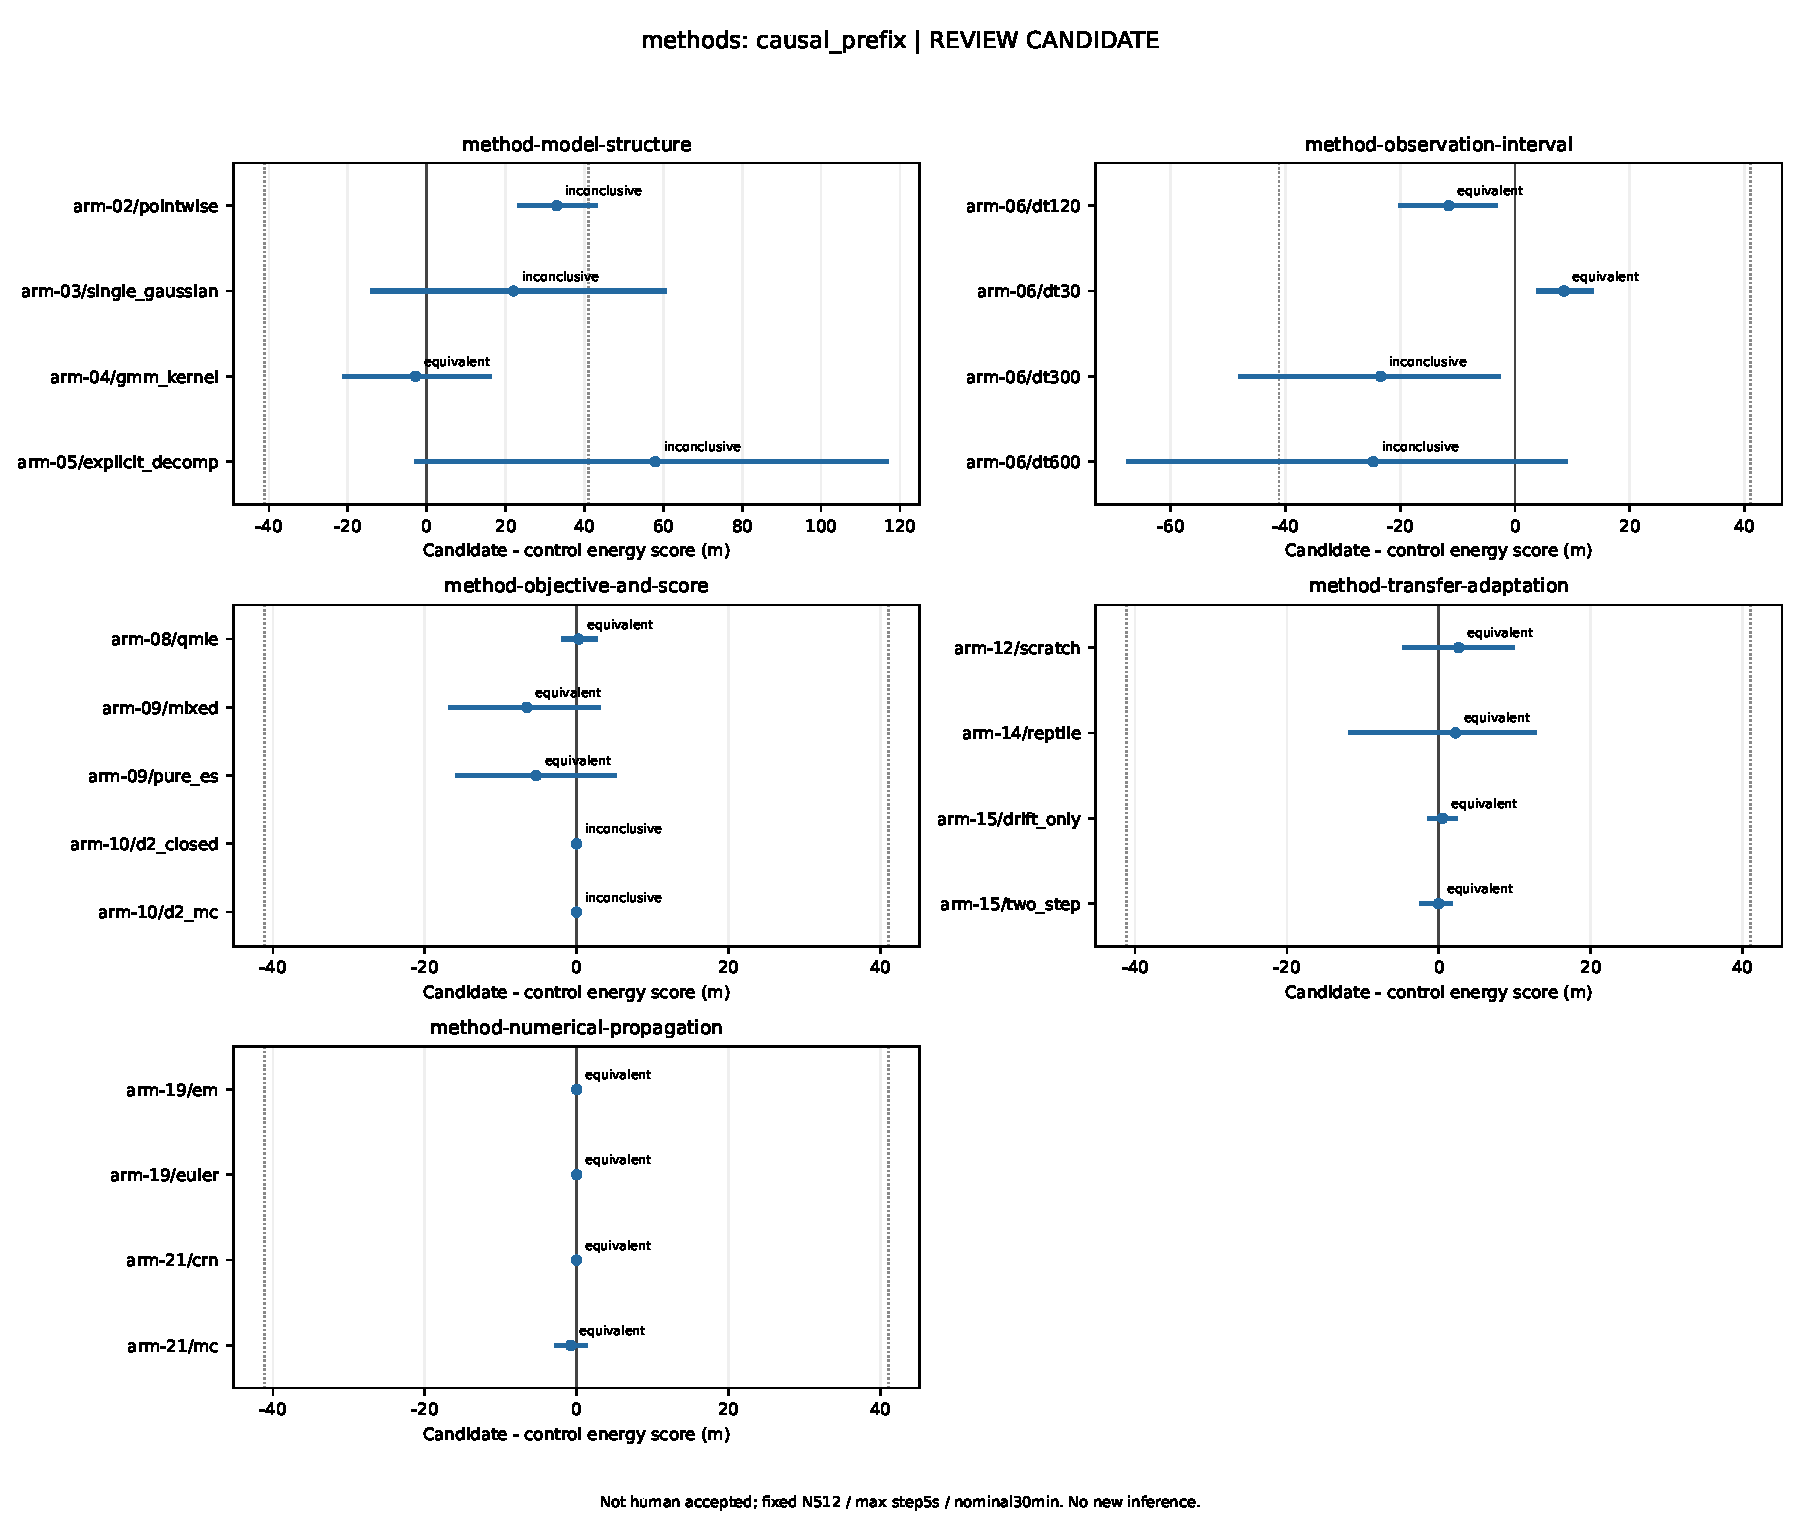
\includegraphics[width=0.96\linewidth,height=0.72\textheight,keepaspectratio]{../final-results-v1/figures/paired-methods-causal_prefix.pdf}
\caption{Actual audit-bound primary method comparison plot.
Intervals and the fixed practical band are retained from the original
analysis. Displayed verdicts are finite-algorithm recorded states, not
resolution-invariant qualification or accepted scientific claims.}
\label{fig:audited-method-comparisons}\hypertarget{fig:audited-method-comparisons}{}
\end{figure}

All 165 original timing records are now present, including 15 excluded
warmups and five trials per cold/warm condition. The 30 condition summaries
retain original values and denominators. Host-interrupted elapsed times
are not corrected or discarded. The archived runtime plot's
\emph{Isolated cold/warm runtime} title is a historical design label,
not certification of uninterrupted isolated latency or speedup;
the clock and interruption limitations in
Section~\ref{sec:runtime-environment} still apply.

The complete anonymous cards, original 16 CSV files, 32 images and 34
bilingual optional table fragments are supplied under
\path{paper/pirc17/final-results-v1/}.
They retain all modes, diagnostic witnesses, trial statuses and units.
The evidence cards bind analysis \texttt{d1d67a3b}, audit
\texttt{8ff917ad} and export \texttt{29cb892f}; full digests and file
manifests are in the package. This is a review delivery, not complete
final manuscript integration or final scientific/human acceptance.
\FloatBarrier



\section{Version and evidence binding}
The methods in this draft were checked against protocol content identity
\path{2267ab84fa77ff4039234a61e8f44be1c3713317d8ad2d1bb4ced9af0c5b293a}
and execution identity
\path{c3e44393f6bc5544aaa21bb273c94eaecb9d0becb4e0590771355c4c0be9b6c2}.
The original completed analysis, saved-output audit, public export and cards
are bound in \path{paper/pirc17/final-results-v1/}; later fixed-budget arithmetic
and card-link checks are in \path{paper/pirc17/qualification-v1/}.
The unchanged complete anonymous input is now published losslessly in
\path{paper/pirc17/replay-input-v1/}. Isolated standard-library commands there
reproduce all six CRPS/endpoint-quantile package files byte-for-byte, not every
original paired verdict, figure and PDF. That complete public rebuild path
remains to be independently verified; source hashes alone cannot replace it.
The executable semantics are in the PIRC-17 modules for direct linear fitting,
causal rollout, metric registry, block inference and evidence-card generation.
An absence of raw private data from this paper is a publication boundary, not
a claim that no independent saved-output audit is needed.


\section{Release and source-reconciliation details}
\label{sec:source-reconciliation-details}\hypertarget{sec:source-reconciliation-details}{}
The following source and bookkeeping descriptions retain the original
reported scope. They add no new data qualification or experiment; the
main text retains the scientific population, input definitions and limitations.

\paragraph{Released identities and development assignment.}
We checked every one of the 7,618 assignments against this frozen source
function and joined every one of the 72,046 sample identities back to its
file, hash and split. The file, recording-hash, segment and sample identity
intersections are zero for each pair of released splits. Counts and source
bindings are in \path{paper/pirc17/partition-description-v1.json}; that identity
reconciliation did not reread raw coordinate, speed or clock values, so it is not a fresh raw-hash,
point-alignment, participant or temporal-independence audit.

For a refined segment with \(n\geq4\) points, the single midpoint sample uses
history indexes \(0,\ldots,\max(1,\lfloor n/2\rfloor-1)\), followed immediately
by target indexes through \(n-1\). All saved bounds satisfy this rule, and
sample identities bind these bounds; each sampled segment has exactly one
sample. This excludes history--target index overlap within that sample, not
physical-time overlap or approximately duplicated tracks across recordings.
The training/adaptation rule is applied to the full released training
sample population before task qualification: sort its 5,251 distinct hash
blocks by SHA256 of \texttt{20260912:} followed by the block ID, assign the
first \(\operatorname{round}(0.8\times5251)=4201\) blocks to training, and the
remaining 1,050 to adaptation. They contain 39,272 and 10,573 windows,
respectively. The selected 328 training windows occupy 259 blocks, 76
adaptation windows occupy 62 blocks, and 81 validation windows occupy 62
blocks. All 16 saved method fits agree with these original roles and window
identities. This does not replace the much smaller actual fitting counts
with the full release counts.

\paragraph{Evaluation-use history.}
The release report records 74 exact recording-hash groups crossing the
\emph{legacy directory} splits; that is a historical reported audit, not the
current zero-intersection assignment above. The bound usage history also
records prior exposure to the 12,370-window released final-evaluation cohort.
The separately used historical GeoLife evaluation had 17,038 windows and is
not a cohort in this protocol. The owner elected on 26 September 2026 to use
the already downloaded data with separated training/evaluation, rather than
create a new untouched holdout. We retain that scope, but do not describe
this evaluation as first-use, design-blind validation. A zero-read declaration
for protocol preparation does not erase historical use or its limits on
claims of independent confirmation.

\paragraph{Saved-speed construction.}
The source construction script converts input km/h to m/s and repeats
the last interval speed at the parent segment's endpoint. That padding and
upstream processing are retained; we do not regenerate or repair speeds.
Its separate \(v_x,v_y\) columns use centered finite differences of local
positions with copied endpoint velocities, so their norm is not the
saved scalar summarized here. We do not estimate speed using the release clock.
All 12,370 original windows have complete finite nonnegative saved
scalars; no window is removed and no failed-stage distribution is replaced
by a successful-subset estimate.

\paragraph{Clock footers and reported anomalies.}
Table~\href{supplement.pdf\#tab:clock-use}{scientific supplement} separates the saved and algorithmic clocks. The
release casts \texttt{t} to \texttt{datetime64[ns]} and integer ticks; the
formal input loader checks exact equality with the qualified source-point
ticks. A dtype or equality check is not a timezone/provenance certificate.
In a fixed first-three-file footer inspection of the original condition
manifest, all three hash-matched files have \texttt{timestamp[ns]} with no
timezone annotation (951, 550 and 794 rows). This limited inspection reads
no point values and does not describe all 7,618 files. A naive timestamp may
have been stored under a UTC convention, but the footer does not establish
that convention. No new timezone correction is inferred or applied.

The original release report records 37,957 duplicate-time intervals in
1,387 segments, 166 backward-time cuts and 10,052 gaps greater than 60
seconds causing cuts. It reports 19,647,139 source condition points,
14,738,300 aligned points and 4,908,839 points not aligned. These are
reported release-reconciliation totals, not fresh pointwise recomputations,
clock error rates or anomaly counts for the selected 46 targets. R1 cleaning,
time refinement and qualification have different denominators; their counts
must not be pooled as one error rate. The legacy observation adapter keeps the
first exact-time duplicate and balances its history/target sides by selecting
existing endpoints. In contrast, the formal visible-prefix loader requires
strictly increasing retained times and does not silently deduplicate a new
prediction input. Metadata, source bindings and the three footer receipts
are in \path{paper/pirc17/clock-description-v1.json}.

\paragraph{Case maps and model asset accounting.}
The private case backgrounds use WorldCover 2021 v200\cite{worldcover2021},
SRTM-labelled Skadi elevation\cite{mapzenterrain}, Overture transportation release 2026-08-19.0
(including OpenStreetMap and TomTom sources)\cite{overture202608,overtureattribution}, and
HydroRIVERS v1\cite{hydrorivers2013,hydroriverslicense}.
These fixed map vintages are not demonstrated to be contemporaneous with
each source trajectory. The route-free acknowledgement record
\path{paper/pirc17/map-source-acknowledgements-v1.json} distinguishes
WorldCover's CC BY 4.0, transportation's ODbL, the SRTM receipt declarations,
and HydroRIVERS' product-specific agreement; it does not assign one common
licence to all layers. HydroRIVERS' prescribed notices and source citations
still require publication review. Map availability and credits do not
establish permission to redistribute private trajectories. Original-route
acquisition permission, privacy review and case publication authorization
remain unverified; this is a disclosure, not an assertion that publication
has been cleared.

The model's retained map catalog is distinct from the three illustrated
backgrounds. Table~\href{supplement.pdf\#tab:model-map-catalog}{scientific supplement} describes the five hash-bound
acquisition receipts and additional raster parents from the frozen feature
snapshot. Counts are admitted files, not assets actually visited, covered
trajectories or successful queries. The same 1283 snapshot parents overlap
1232 receipt assets; only 51 add files to the 1354-file receipt catalog.
The resulting 1405-file catalog does not guarantee support at predicted positions.

\paragraph{Product references and upstream provenance.}
The model's elevation channel labelled \texttt{srtm} uses the Mapzen AWS
Skadi distribution\cite{mapzenterrain}; the separate admitted Copernicus
channel is GLO-30 Public, 2021 release\cite{copernicusdem2021}.
WorldCover v200\cite{worldcover2021}, Overture release
2026-08-19.0\cite{overture202608}, and HydroRIVERS v1.0\cite{hydrorivers2013,hydroriverslicense}
identify the other model-input products, not just case backgrounds.
The Skadi format documentation describes a distribution using SRTM and
other open elevation sources. The receipt's GL1 label and 2000 interval
therefore do not certify pure NASA SRTM provenance or acquisition year for
every retained tile. We retain the frozen asset hashes and receipt labels;
the cited documentation revision is not a newly assigned data release.
Provider attribution documents\cite{mapzenattribution,overtureattribution,hydroriverslicense}
are distinct from product and methodological references. Their consultation
does not clear tile-specific obligations or private-route publication.
Documentation access dates are not acquisition dates or immutable data
versions; missing per-tile upstream identities remain a limitation.


\section{Scoring and execution capture times}
\label{sec:score-execution-snapshots}\hypertarget{sec:score-execution-snapshots}{}
The scoring snapshot captured on 6 October 2026 at 00:54:18.683579 UTC
contains 10384 successful scientific
score rows, five failure rows and 631 missing rows from the registered 11020
forecasts. These are captured scoring dispositions, not a real-time forecast
counter. The entire primary method grid is complete: 28 configurations,
46 recording-hash blocks and five forecast RNG seeds give 6440 score rows.
Each configuration has 230 rows, but the recording-block count is 46.
No forecast, refit or particle scoring was performed for this snapshot.
Its precise capture time and input hashes are retained in
\path{paper/pirc17/preliminary-method-statistics-v1.json}.
The execution census in Section~\ref{sec:execution-coverage} was captured
later, at 06:53:13.846553 UTC; its success count is 130 higher.
These are different dated snapshots, not two simultaneous counters.
Their item-level difference has not been independently audited here.

Table~\ref{tab:capture-count-difference} reconciles the two saved summaries
on the identical 114 configuration--origin-mode cells. All 22 cells with
changed counts belong to the terrain matrix: their net success increases
are 57 for causal prefixes, 8 for known velocity and 65 for point-only
origins. In each cell the success increase equals the decrease in missing
counts, and the failed count is unchanged. All 84 method cells are
unchanged. Thus the 130-count difference does not add observations to the
6440-row primary method result tables or change their pinned input version.
The corresponding abstract and method findings retain the earlier scoring
snapshot; the completeness tables retain the later execution census.

\begin{table}[htbp]
\centering\small
\caption{Reconciliation of saved success counts, not a reconstruction of
individual forecast membership. Earlier means the 00:54 scoring summary;
later means the 06:53 execution census on 6 October 2026.}
\label{tab:capture-count-difference}\hypertarget{tab:capture-count-difference}{}
\begin{tabular}{@{}llrrr@{}}
\toprule
Matrix & Origin mode & Earlier & Later & Net change\\
\midrule
Methods & Causal prefix & 6440 & 6440 & 0\\
Methods & Known velocity & 838 & 838 & 0\\
Methods & Point only & 840 & 840 & 0\\
Terrain & Causal prefix & 1974 & 2031 & 57\\
Terrain & Known velocity & 292 & 300 & 8\\
Terrain & Point only & 0 & 65 & 65\\
\midrule
Total & & 10384 & 10514 & 130\\
\bottomrule
\end{tabular}
\end{table}

The route-free \path{paper/pirc17/capture-count-reconciliation-v1.json}
retains every cell's two count triples, exact capture times and input file
hashes. Neither original summary retains the per-item work-ID sets.
Consequently a net increase of 130 is not a verified set of 130 new item
identities: membership replacement within a cell cannot be ruled out by
these counts. This count reconciliation neither replaces the original
saved-output audit nor establishes payload integrity, independence or
scientific qualification. No source snapshot or statistical result is
overwritten, and no prediction, score or resampling is added.

\clearpage

\section{Captured forecast and family completeness}
\label{sec:execution-coverage}\hypertarget{sec:execution-coverage}{}
Table~\ref{tab:execution-coverage} is a captured execution census at
6 October 2026, 06:53 UTC, not a new accuracy analysis. It reads only the
original workload, prediction and score-cache indexes, including exact
saved-source bindings. It neither loads prediction arrays nor re-estimates
scores. All 11020 planned scientific forecasts retain their original
configuration, origin-mode and five-seed denominator. At capture, 10514 were
successful, 501 still runnable and five failed; their score indexes had
the same counts, with no invalid bindings detected. An indexed success is
not independent validation of the score payload or scientific qualification.

\begin{table}[htbp]
\centering\small
\caption{Unique planned forecasts by matrix and origin mode at the captured
time. These six rows sum to 11020; origin modes reuse blocks, not new people.}
\label{tab:execution-coverage}\hypertarget{tab:execution-coverage}{}
\begin{tabular}{@{}llrrrr@{}}
\toprule
Matrix & Origin mode & Planned & Successful & Runnable & Failed\\
\midrule
Methods & Causal prefix & 6440 & 6440 & 0 & 0\\
Methods & Known velocity & 840 & 838 & 0 & 2\\
Methods & Point only & 840 & 840 & 0 & 0\\
Terrain & Causal prefix & 2300 & 2031 & 266 & 3\\
Terrain & Known velocity & 300 & 300 & 0 & 0\\
Terrain & Point only & 300 & 65 & 235 & 0\\
\midrule
Total & & 11020 & 10514 & 501 & 5\\
\bottomrule
\end{tabular}
\end{table}

The method results in Section~\href{supplement.pdf\#sec:method-results}{scientific supplement} concern the complete $28\times46\times5=6440$
primary grid, not a mean over all matrices and modes. Known-velocity and
point-only cases each reuse the first six primary blocks and are bounded
descriptive initialization diagnostics. The known-velocity failures are in
\texttt{single\_gaussian} and \texttt{dt30}; the primary terrain failures are
in \texttt{all-terrain}, \texttt{lio-road} and \texttt{lio-river}.
They are retained, not retried automatically or omitted from denominators.

\begin{table}[htbp]
\centering\small
\caption{Required primary score-index rows in each registered comparison
family at the same capture. Complete means index-complete only. Missing or
failed rows prevent a complete paired comparison; families overlap.}
\label{tab:family-coverage}\hypertarget{tab:family-coverage}{}
\begin{tabular}{@{}lrrrrl@{}}
\toprule
Primary family & Required & Success & Missing & Failed & Disposition\\
\midrule
Model structure & 1150 & 1150 & 0 & 0 & Complete index\\
Observation interval & 1150 & 1150 & 0 & 0 & Complete index\\
Objective and score & 1380 & 1380 & 0 & 0 & Complete index\\
Training and adaptation & 1150 & 1150 & 0 & 0 & Complete index\\
Numerical propagation & 1380 & 1380 & 0 & 0 & Complete index\\
Terrain all/LOO & 1380 & 1219 & 160 & 1 & Unavailable\\
Terrain LIO & 1150 & 1017 & 131 & 2 & Unavailable\\
\bottomrule
\end{tabular}
\end{table}

Table~\ref{tab:family-coverage} counts the unique required configuration rows
within each family, not one new set of observations per contrast. Shared
controls appear in more than one family, so its rows cannot be summed into
an experiment total. In particular, the terrain families share 230 baseline
rows; their 160 and 131 missing scores include 25 shared baseline rows and
therefore represent 266 unique primary missing forecasts, not 291.
Index completion does not waive the independent saved-output audit,
mechanism evidence, uncertainty checks or final acceptance. No effect
estimate is obtained from a failed family's successful intersection.

The 501 remaining scientific forecasts are separate from the 261 scheduled
auxiliaries: 58 inertial paths, 38 replays, 75 cold timings, 15 excluded
warm-ups and 75 warm timings. None of those auxiliaries had completed at
capture; 290 same-grid references had already completed. Warm-up measurements
are excluded from the measured runtime sample. Cost conclusions must use
the original timing protocol, not scientific prediction counts or this census.



\Needspace{.70\textheight}

\Needspace{.70\textheight}



\section{Detailed CPU environment records}
\label{sec:runtime-record-details}\hypertarget{sec:runtime-record-details}{}
Recorded threads are PyTorch 6/inter-op 12, OMP/MKL 6 and OpenBLAS/Numba 12.
Library thread counts are not prediction-worker counts. The machine descriptor
identifies Intel family/model/stepping, not a verified marketing CPU model.
The public reader projection binds the original environment digest and removes
workstation/DLL paths.

Each isolated CPU trial carries the original digest of a hardware manifest:
platform and processor reports, logical and physical CPU counts, total RAM,
Python, NumPy, PyTorch and psutil versions, and versions of available DuckDB,
Numba, Rasterio and PyArrow packages. It also records PyTorch thread counters,
Numba's thread count if loaded, and configured OMP, MKL, OpenBLAS and Numba
thread-environment variables. An unset variable does not imply a single thread.
The public hardware entry is keyed by the original full-manifest digest and
omits loaded native-threadpool records that can contain local DLL paths.
Final hardware values must come from the audited timing records, not the
machine that compiles this draft. The timing protocol's ``warm OS cache''
wording is not a measured cache-state guarantee: trials do not flush,
control or record OS cache occupancy. The original timing receipts and
their definitions are retained, not relabelled or remeasured.


\section{Execution records and reconstruction}
\label{sec:execution-reconstruction}\hypertarget{sec:execution-reconstruction}{}
During continuation, the two workers process disjoint original task identities.
Each owns its mutable map-query and history state; one dispatcher writes
atomic completion metadata. Thirty-minute monitoring records overall
success/failure/remaining counts and separate worker increments. These are
execution observations, not model-quality scores or additional experiments.

The closed saved-score inventory and the original scientific-task metadata
agree on the terminal counts in Table~\ref{tab:terminal-score-inventory}.
The 8120 method forecasts and 2900 terrain forecasts total 11020 scientific
workloads. The common-score grid additionally includes 290 registered
same-grid references and 58 deterministic inertial paths; it therefore has
$58\{5(28+10+1)+1\}=11368$ slots, not 11368 independent observations.
There are 46 primary and 12 support blocks. A failed forecast retains a failed
score slot, not a zero-valued error. Counts do not repair the four unavailable
comparison families or establish that every score agrees with the raw output.

\begin{table}[htbp]\centering\small
\caption{Terminal saved-score inventory, inspected 8 October 2026.
Expected counts retain all registered slots; success/failure are saved
dispositions, not scientific qualification. References are outside the
11020 scientific-forecast denominator.}\label{tab:terminal-score-inventory}\hypertarget{tab:terminal-score-inventory}{}
\begin{tabular}{@{}lrrr@{}}\toprule
Role & Expected & Successful & Failed\\\midrule
Method forecasts & 8120 & 8118 & 2\\
Terrain forecasts & 2900 & 2897 & 3\\
Scientific subtotal & 11020 & 11015 & 5\\
Same-grid references & 290 & 290 & 0\\
Inertial paths & 58 & 58 & 0\\
Common-score total & 11368 & 11363 & 5\\
\bottomrule\end{tabular}\end{table}

Common scoring has closed all 11368 rows and 58 blocks; all 261 original
auxiliary tasks and the independent saved-output replay have completed.
The once-only original analysis and audit are retained unchanged. Public
export and evidence-card construction have completed without new forecasts,
fits or a repeated audit. Section~\ref{sec:audited-review-update} identifies
the current complete review package. The public consumer produces sixteen tables
and sixteen figures in PNG and PDF, retaining the original estimates,
intervals, missingness and units. Registered aggregate exports omit private trajectories,
targets, coordinates, model weights and local machine paths. Their content
identities and rendering environment permit an independent reconstruction
without reopening private data.

Reproduction has three distinct scopes. Rebuilding the manuscript compiles
the declared English and Chinese sources and resolves their references;
it does not repeat forecasts. Regenerating public tables and figures consumes
the hash-bound evidence cards, copies the original numerical estimates and
retains explicit unavailable cells, without new bootstrap draws or tests.
Scientific reproduction additionally checks saved forecast outputs and their
source bindings through the independent audit. A successful PDF build cannot
replace that audit or authorize an empirical claim.

The final review record will identify the immutable public export and cards,
their input manifest, protocol and execution, renderer versions and exact
manuscript revision. Figure byte equality is limited to the recorded library
and font environment; arbitrary TeX installations need not produce identical
PDF bytes. Historical manuscripts remain separately named, and their existing
release workflow is not evidence that this PIRC-17 draft has been approved
or published. Final authorship and acceptance remain explicit human decisions.


